\input{mmd-article-header}
\def\mytitle{Cloud Foundry Technical Overview}
\def\myauthor{VMware 2012 - Cloud Foundry}
\def\latexmode{memoir}
\input{mmd-article-begin-doc}
\chapter{Introduction}
\label{introduction}

Cloud Foundry BOSH is an open source tool chain for release engineering, deployment and life cycle management of cloud-scale distributed services. In this manual we describe the architecture, topology, configuration, and use of BOSH, as well as the structure and conventions used in packaging and deployment.

\chapter{Managing Distributed Services}
\label{managingdistributedservices}

BOSH was originally developed in the context of the Cloud Foundry Application Platform as a Service, but even if this has been the primary consumer, the framework is general purpose and can be used to deploy other distributed services on top of a Cloud Provider Interface (CPI) provided by VMware vSphere, Amazon Web Services, or OpenStack. 

\chapter{BOSH Components}
\label{boshcomponents}

\section{Fig 1. Interaction of BOSH Components}
\label{fig1.interactionofboshcomponents}

\begin{figure}[htbp]
\centering
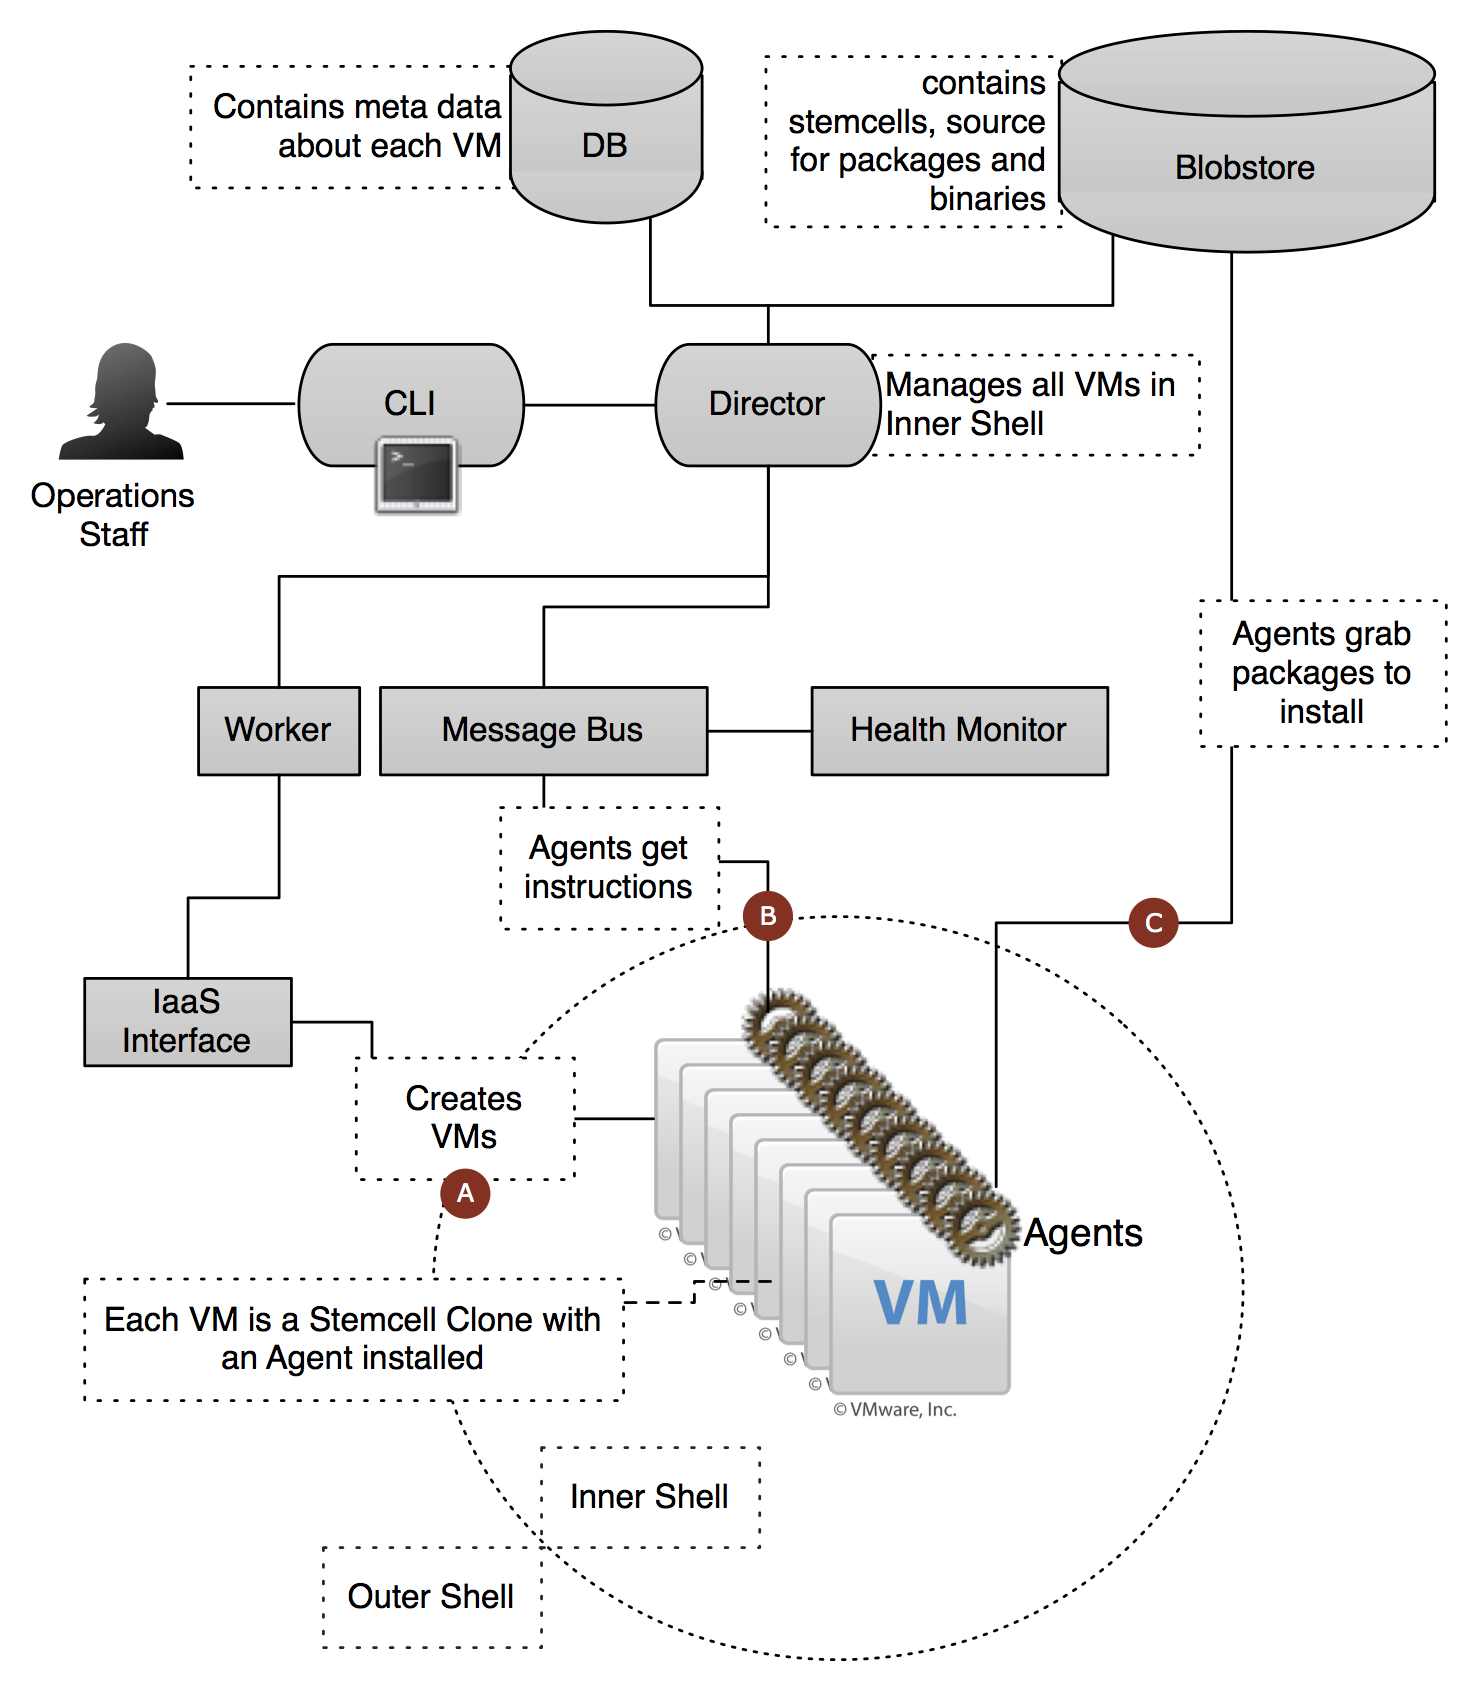
\includegraphics[keepaspectratio,width=\textwidth,height=0.75\textheight]{fig1.png}
\caption{Figure 1}
\label{}
\end{figure}


\section{Infrastructure as a Service (IaaS)}
\label{infrastructureasaserviceiaas}

The core BOSH engine is abstracted away from any particular Infrastructure as a Service (IaaS), such as VMware vSphere, AWS or OpenStack. IaaS interfaces are implemented as plugins to BOSH. Currently, BOSH supports both VMware vSphere and Amazon Web Services. Virtual Machines (VMs) are created and destroyed through Workers, which are sent instructions from the Director. Those VMs are created based on a \textbf{Stemcell} that is uploaded to BOSH's Blobstore through the Command Line Interface (CLI).

\section{Cloud Provider Interface (CPI)}
\label{cloudproviderinterfacecpi}

As a user of BOSH you're not directly exposed to the the BOSH Cloud Provider Interface, but it can be helpful to understand its primitives when learning how BOSH works. The current examples of these interfaces are in: \texttt{bosh\slash vsphere\_cpi\slash lib\slash cloud\slash vsphere\slash cloud.rb} for vSphere, and \texttt{bosh\slash aws\_cpi\slash lib\slash cloud\slash aws\slash cloud.rb} for Amazon Web Services. Within those subdirectories are Ruby classes with methods to do the following: 

\begin{itemize}
\item create\_stemcell

\item delete\_stemcell

\item create\_vm

\item delete\_vm

\item reboot\_vm

\item configure\_networks

\item create\_disk

\item delete\_disk

\item attach\_disk

\item detach\_disk

\end{itemize}

In addition to these methods are others specific to each cloud interface. For example, the Amazon Web Services interface includes methods for Elastic Block Store, which are unnecessary on vSphere. Please refer to the API documentation in the files listed above for a detailed explanation of the CPI primitives.

The CPI is used primarily to do low level creation and management of resources in an IaaS. Once a resource is up and running, command and control is handed over to the higher level BOSH Director-Agent interaction.

\section{BOSH Director}
\label{director}

The Director is the core orchestrating component in BOSH which controls creation of VMs, deployment, and other life cycle events of software and services.

\section{BOSH CLI}
\label{boshcli}

The BOSH Command Line Interface is the mechanism for users to interact with BOSH using a terminal session. BOSH commands follow the format shown below:

\begin{adjustwidth}{2.5em}{2.5em}
\begin{verbatim}

$bosh [--verbose] [--config|-c <FILE>] [--cache-dir <DIR>]
        [--force] [--no-color] [--skip-director-checks] [--quiet]
        [--non-interactive]

\end{verbatim}
\end{adjustwidth}

A full overview of BOSH commands and installation appears in the BOSH CLI (\autoref{bosh_cli}) and BOSH installation (\autoref{bosh_install}) sections.

\section{Stemcells}
\label{stemcells}

A BOSH Stemcell is a VM template with an embedded BOSH Agent. The Stemcell used for Cloud Foundry is a standard Ubuntu distribution. Stemcells are uploaded using the BOSH CLI and used by the Director when creating VMs through the CPI. When the Director creates a VM through the CPI, it will pass along configurations for networking and storage, as well as the location and credentials for the BOSH Message Bus and the BOSH Blobstore.

\section{Agent}
\label{agent}

When a Stemcell is created, it is comprised of the barebones operating system (Ubuntu in the case of Cloud Foundry) and an Agent. The Agent listens for instructions from the Director and performs operations on the VM according to these instructions. A typical instruction would be to download and install new packages from the Blobstore.

\section{Releases}
\label{releases}

A Release in BOSH is a packaged bundle of service descriptors known as Jobs. Jobs are collections of software bits and configurations. Any given Release contains all the static bits (source or binary) required to have BOSH manage an application or a distributed service. 

A Release is typically not restricted to any particular environment. As such, it can be re-used across clusters handling different stages in a service life cycle, such as Development, QA, Staging, or Production. The BOSH CLI manages both the creation of Releases and their deployments into specific environments.

\section{Deployments}
\label{deployments}

While BOSH Stemcells and Releases are static components, we say that they are bound together into a Deployment by a Deployment Manifest. In the Deployment Manifest, you declare pools of VMs, which networks they live on, and which Jobs (service components) from the Release you want to activate. Job configurations specify life cycle parameters, the number of instances of a Job, and network and storage requirements. Furthermore, the Deployment Manifest allows you to specify properties used to parameterize configuration templates contained in the Release.

Using the BOSH CLI, you specify a Deployment Manifest and perform a Deploy operation (\texttt{bosh deploy}), which creates or updates resources on your cluster according to your specifications.

\section{Blobstore}
\label{blobstore}

The BOSH Blobstore is used to store the content of Releases (BOSH Jobs (\autoref{jobs}) and Packages (\autoref{packages}) in their source form as well as the compiled image of BOSH Packages). Releases (\autoref{releases}) are uploaded by the BOSH CLI and inserted into the Blobstore by the BOSH Director. When you deploy a Release, BOSH will orchestrate the compilation of packages and store the result in the Blobstore. When BOSH deploys a BOSH Job to a VM, the BOSH Agent will pull the specified Job and associated BOSH Packages from the Blobstore.

BOSH also uses the Blobstore as an intermediate store for large payloads, such as log files (see BOSH logs) and output from the BOSH Agent that exceeds the max size for messages over the message bus.

There are currently three Blobstores supported in BOSH:

\begin{enumerate}
\item \href{http://www.emc.com/storage/atmos/atmos.htm}{Atmos}\footnote{\href{http://www.emc.com/storage/atmos/atmos.htm}{http:/\slash www.emc.com\slash storage\slash atmos\slash atmos.htm}}

\item \href{http://aws.amazon.com/s3/}{S3}\footnote{\href{http://aws.amazon.com/s3/}{http:/\slash aws.amazon.com\slash s3\slash }}

\item \href{https://github.com/cloudfoundry/bosh/tree/master/simple_blobstore_server}{simple blobstore server}\footnote{\href{https://github.com/cloudfoundry/bosh/tree/master/simple_blobstore_server}{https:/\slash github.com\slash cloudfoundry\slash bosh\slash tree\slash master\slash simple\_blobstore\_server}}

\end{enumerate}

The default BOSH configuration uses the simple blobstore server, as the load is very light and low latency is preferred.

\section{Health Monitor}
\label{healthmonitor}

The BOSH (Health) Monitor receives health status and life cycle events from the BOSH Agents and can through notification plugins (such as email), notify if components are in an unexpected state. It has a simple awareness of events in the system, so as to not alert if a component is updated.

\section{Message bus}
\label{messagebus}

BOSH uses the \href{http://github.com/dcollison/nats}{NATS}\footnote{\href{http://github.com/dcollison/nats}{http:/\slash github.com\slash dcollison\slash nats}} message bus for command and control.

\chapter{Using BOSH}
\label{usingbosh}

Before we can use BOSH we need to install the BOSH CLI. You will need a running development environment with an uploaded Stemcell. You can learn about those steps in the BOSH Installation (\autoref{boshinstallation}) section.

\section{Installing BOSH Command Line Interface}
\label{bosh_install}

The following steps install BOSH CLI on Ubuntu 10.04 LTS. You can install on either a physical or Virtual Machine.

\subsection{Install Ruby via rbenv}
\label{installrubyviarbenv}

\begin{enumerate}
\item Bosh is written in Ruby. Let's install Ruby's dependencies

\begin{verbatim}
sudo apt-get install git-core build-essential libsqlite3-dev curl libmysqlclient-dev libxml2-dev libxslt-dev libpq-dev
\end{verbatim}


\item Get the latest version of rbenv

\begin{verbatim}
cd
git clone git://github.com/sstephenson/rbenv.git .rbenv
\end{verbatim}


\item Add \texttt{\ensuremath{\sim}\slash .rbenv\slash bin} to your \texttt{\$PATH} for access to the \texttt{rbenv} command-line utility

\begin{verbatim}
echo 'export PATH="$HOME/.rbenv/bin:$PATH"' >> ~/.bash_profile
\end{verbatim}


\item Add rbenv init to your shell to enable shims and autocompletion

\begin{verbatim}
echo 'eval "$(rbenv init -)"' >> ~/.bash_profile
\end{verbatim}


\item Download Ruby 1.9.2
\emph{Note: You can also build ruby using ruby-build plugin for rbenv. See https:/\slash github.com\slash sstephenson\slash ruby-build}

\begin{verbatim}
wget http://ftp.ruby-lang.org/pub/ruby/1.9/ruby-1.9.2-p290.tar.gz
\end{verbatim}


\item Unpack and install Ruby

\begin{verbatim}
 tar xvfz ruby-1.9.2-p290.tar.gz
 cd ruby-1.9.2-p290
 ./configure --prefix=$HOME/.rbenv/versions/1.9.2-p290
 make
 make install
\end{verbatim}


\item Restart your shell so the path changes take effect

\begin{verbatim}
source ~/.bash_profile
\end{verbatim}


\item Set your default Ruby to be version 1.9.2

\begin{verbatim}
rbenv global 1.9.2-p290
\end{verbatim}


\item Update rubygems and install bundler. \emph{Note: After installing gems (\texttt{gem install} or \texttt{bundle install}) run \texttt{rbenv rehash} to add new shims}

\begin{verbatim}
gem update --system
gem install bundler
rbenv rehash
\end{verbatim}


\end{enumerate}

\subsection{Install Local BOSH and BOSH Releases}
\label{installlocalboshandboshreleases}

\begin{enumerate}
\item Sign up for the Cloud Foundry Gerrit server at \href{http://reviews.cloudfoundry.org}{http:/\slash reviews.cloudfoundry.org}\footnote{\href{http://reviews.cloudfoundry.org}{http:/\slash reviews.cloudfoundry.org}}

\item Set up your ssh public key (accept all defaults)

\begin{verbatim}
ssh-keygen -t rsa
\end{verbatim}


\item Copy your key from \texttt{\ensuremath{\sim}\slash .ssh\slash id\_rsa.pub} into your Gerrit account

\item Create \ensuremath{\sim}\slash .gitconfig as follows (Make sure that the email specified is registered with gerrit):

\begin{verbatim}
[user]
name = YOUR_NAME
email = YOUR_EMAIL
[alias]
gerrit-clone = !bash -c 'gerrit-clone $@' -
\end{verbatim}


\item Clone gerrit tools using git

\begin{verbatim}
git clone git@github.com:vmware-ac/tools.git
\end{verbatim}


\end{enumerate}

\textbf{NOTE: PUBLIC TOOLS REPO IN FINAL DRAFT}

\begin{enumerate}
\item Add gerrit-clone to your path

\begin{verbatim}
echo 'export PATH="$HOME/tools/gerrit/:$PATH"' >> ~/.bash_profile
\end{verbatim}


\item Restart your shell so the path changes take effect

\begin{verbatim}
source ~/.bash_profile
\end{verbatim}


\item Clone BOSH repositories from Gerrit

\begin{verbatim}
git gerrit-clone ssh://reviews.cloudfoundry.org:29418/release.git
git gerrit-clone ssh://reviews.cloudfoundry.org:29418/bosh.git
\end{verbatim}


\item Run some rake tasks to install the BOSH CLI

\begin{verbatim}
cd ~/bosh
rake bundle_install (Note: if this fails run 'gem pristine rake' and retry)
cd cli
bundle exec rake build
gem install pkg/bosh_cli-x.x.x.gem
rbenv rehash
\end{verbatim}


\end{enumerate}

\subsection{Deploy to your BOSH Environment}
\label{deploytoyourboshenvironment}

With a fully configured environment, we can begin deploying a Cloud Foundry Release to our environment. As listed in the prerequisites, you should already have an environment running, as well as the IP address of the BOSH Director. To set this up, skip to the BOSH Installation (\autoref{boshinstallation}) section.

\subsection{Point BOSH at a Target and Clean your Environment}
\label{pointboshatatargetandcleanyourenvironment}

\begin{enumerate}
\item Target your Director (this IP is an example.) \textbf{NOTE: EXAMPLE WORKS FOR INTERNAL USE (u: admin \slash  p: admin)}

\begin{verbatim}
bosh target 11.23.128.219:25555 
\end{verbatim}


\item Check the state of your BOSH settings.

\begin{verbatim}
bosh status
\end{verbatim}


\item The result of your status will be akin to:

\begin{verbatim}
Target         dev48 (http://11.23.128.219:25555) Ver: 0.3.12 (01169817)
UUID           4a8a029c-f0ae-49a2-b016-c8f47aa1ac85
User           admin
Deployment     not set
\end{verbatim}


\item List any previous Deployments (we will remove them in a moment). If this is your first Deployment, there will be none listed.

\begin{verbatim}
bosh deployments
\end{verbatim}


\item The result of \texttt{bosh deployments} should be akin to:

\begin{verbatim}
+-------+
| Name  |
+-------+
| dev48 |
+-------+
\end{verbatim}


\item Delete the existing Deployments (ex: dev48.) 

\begin{verbatim}
bosh delete deployment dev48
\end{verbatim}


\item Answer \texttt{yes} to the prompt and wait for the deletion to complete.

\item List previous Releases (we will remove them in a moment). If this is your first Deployment, there will be none listed.

\begin{verbatim}
bosh releases
\end{verbatim}


\item The result of \texttt{bosh releases} should be akin to:

\begin{verbatim}
+---------------+---------------+
| Name          | Versions      |
+---------------+---------------+
| cloudfoundry  | 47, 55, 58    |
+---------------+---------------+
\end{verbatim}


\item Delete the existing Releases (ex: cloudfoundry) 

\begin{verbatim}
bosh delete release cloudfoundry
\end{verbatim}


\item Answer \texttt{yes} to the prompt and wait for the deletion to complete.

\end{enumerate}

\subsection{Create a Release}
\label{createarelease}

\begin{enumerate}
\item Change directories into the release directory.

\end{enumerate}

\textbf{NOTE: This is not correct yet - Get correct locations and names from Oleg}

\begin{adjustwidth}{2.5em}{2.5em}
\begin{verbatim}

    cd ~/release

This directory contains the Cloud Foundry deployment and release files.

\end{verbatim}
\end{adjustwidth}

\begin{enumerate}
\item Reset your environment

\begin{verbatim}
bosh reset release
\end{verbatim}


\item Answer \texttt{yes} to the prompt and wait for the environment to be reset

\item Create a Release

\begin{verbatim}
bosh create release --force --with-tarball
\end{verbatim}


\item Answer \texttt{cloudfoundry} to the \texttt{release name} prompt

\item Your terminal will display information about the release including the Release Manifest, Packages, Jobs, and tarball location.

\item Open \texttt{bosh-sample-release\slash cloudfoundry.yml} in your favorite text editor and confirm that \texttt{name} is \texttt{cloudfoundry} and \texttt{version} matches the version that was displayed in your terminal (if this is your first release, this will be version 1.)

\end{enumerate}

\subsection{Deploy the Release}
\label{deploytherelease}

\begin{enumerate}
\item Upload the cloudfoundry Release to your Environment.

\begin{verbatim}
bosh upload release dev_releases/cloudfoundry-1.tgz
\end{verbatim}


\item Your terminal will display information about the upload, and an upload progress bar will reach 100\% after a few minutes.

\item Open \texttt{releases\slash cloudfoundry.yml} and make sure that your network settings match the environment that you were given.

\item Deploy the Release.

\begin{verbatim}
bosh deploy
\end{verbatim}


\item Your deployment will take a few minutes.

\item You may now target the Cloud Foundry deployment using VMC, as described in the Cloud Foundry documentation.

\end{enumerate}

\chapter{BOSH Installation}
\label{boshinstallation}

Deploying BOSH is a two step process. First, The BOSH Deployer is used to deploy a micro BOSH, which will live in a single virtual machine. The second step is to use the micro BOSH as a means to deploy the final, distributed production BOSH on multiple VMs. The graphic below illustrates this two step process.

\textbf{NOTE: Matt will create a graphic for this}

\section{Prerequisites}
\label{prerequisites}

\begin{enumerate}
\item It is recommend that you install into an empty gemset (or similar.)

\item Install some core packages on Ubuntu.

\begin{verbatim}
% sudo apt-get -y install libsqlite3-dev genisoimage
\end{verbatim}


\item Build the BOSH Deployer.

\begin{verbatim}
% cd bosh/deployer
% bundle install
% rake install
\end{verbatim}


\end{enumerate}

Once you have installed micro BOSH, you will see some extra commands appear after typing \texttt{bosh} on your command line. 

\textbf{The \texttt{bosh micro} commands must also be run within the deployments directory}

\begin{adjustwidth}{2.5em}{2.5em}
\begin{verbatim}

    % bosh help
    ...
    Micro
        micro deployment [<name>] Choose micro deployment to work with
        micro status              Display micro BOSH deployment status
        micro deployments         Show the list of deployments
        micro deploy <stemcell>   Deploy a micro BOSH instance to the currently
                        selected deployment
                        --update   update existing instance
        micro delete              Delete micro BOSH instance (including
                        persistent disk)
        micro agent <args>        Send agent messages
        micro apply <spec>        Apply spec

\end{verbatim}
\end{adjustwidth}

\section{Configuration}
\label{configuration}

For a minimal configuration example, see: \texttt{deployer\slash spec\slash assets\slash test-bootstrap-config.yml}. Note that \texttt{disk\_path} is \texttt{BOSH\_Deployer} rather than \texttt{BOSH\_Disks}. A datastore folder other than \texttt{BOSH\_Disks} is required if your vCenter hosts other Directors. The \texttt{disk\_path} folder needs to be created manually. Also, your configuration must live inside a \texttt{deployments} directory and follow the convention of having a \texttt{\$name} subdir containing \texttt{micro\_bosh.yml}, where \texttt{\$name} is your Deployment name. 

For example:

\begin{adjustwidth}{2.5em}{2.5em}
\begin{verbatim}

    % find deployments -name micro_bosh.yml
    deployments/vcs01/micro_bosh.yml
    deployments/dev32/micro_bosh.yml
    deployments/dev33/micro_bosh.yml

\end{verbatim}
\end{adjustwidth}

Deployment state is persisted to deployments\slash bosh-deployments.yml.

\section{Deployment}
\label{deployment}

\begin{enumerate}
\item Download a micro BOSH stemcell:

\begin{verbatim}
% mkdir -p ~/stemcells
% cd stemcells
% bosh public stemcells
+-------------------------------+----------------------------------------------------+
| Name                          | Url                                                |
+-------------------------------+----------------------------------------------------+
| bosh-stemcell-0.4.7.tgz       | https://blob.cfblob.com/rest/objects/4e4e7...h120= |
| micro-bosh-stemcell-0.1.0.tgz | https://blob.cfblob.com/rest/objects/4e4e7...5Mms= |
| bosh-stemcell-0.3.0.tgz       | https://blob.cfblob.com/rest/objects/4e4e7...mw1w= |
| bosh-stemcell-0.4.4.tgz       | https://blob.cfblob.com/rest/objects/4e4e7...r144= |
+-------------------------------+----------------------------------------------------+
To download use 'bosh download public stemcell <stemcell_name>'.
% bosh download public stemcell micro-bosh-stemcell-0.1.0.tgz
\end{verbatim}


\item Set the micro BOSH Deployment using:

\begin{verbatim}
% cd /var/vcap/deployments
% bosh micro deployment dev33
Deployment set to '/var/vcap/deployments/dev33/micro_bosh.yml'
\end{verbatim}


\item Deploy a new micro BOSH instance and create a new persistent disk.

\begin{verbatim}
% bosh micro deploy ~/stemcells/micro-bosh-stemcell-0.1.0.tgz
\end{verbatim}


\item Update an existing micro BOSH instance. The existing persistent disk will be attached to the new VM.

\begin{verbatim}
% bosh micro deploy ~/stemcells/micro-bosh-stemcell-0.1.1.tgz --update
\end{verbatim}


\end{enumerate}

\section{Deleting a micro BOSH deployment}
\label{deletingamicroboshdeployment}

The \texttt{delete} command will delete the VM, Stemcell and persistent disk.

Example:

\begin{adjustwidth}{2.5em}{2.5em}
\begin{verbatim}

    % bosh micro delete

\end{verbatim}
\end{adjustwidth}

\section{Checking Status of a micro BOSH deploy}
\label{checkingstatusofamicroboshdeploy}

The status command will show the persisted state for a given micro BOSH instance.

\begin{adjustwidth}{2.5em}{2.5em}
\begin{verbatim}

    % bosh micro status
    Stemcell CID   sc-f2430bf9-666d-4034-9028-abf9040f0edf
    Stemcell name  micro-bosh-stemcell-0.1.0
    VM CID         vm-9cc859a4-2d51-43ca-8dd5-220425518fd8
    Disk CID       1
    Deployment     /var/vcap/deployments/dev33/micro_bosh.yml
    Target         micro (http://11.23.194.100:25555) Ver: 0.3.12 (00000000)

\end{verbatim}
\end{adjustwidth}

\section{Listing Deployments}
\label{listingdeployments}

The \texttt{deployments} command prints a table view of deployments\slash bosh-deployments.yml.

\begin{adjustwidth}{2.5em}{2.5em}
\begin{verbatim}

    % bosh micro deployments

\end{verbatim}
\end{adjustwidth}

\section{Applying a specification}
\label{applyingaspecification}

The micro-bosh-stemcell includes an embedded \texttt{apply\_spec.yml}. This command can be used to apply a different spec to an existing instance. The \texttt{apply\_spec.yml} properties are merged with your Deployment's network.ip and cloud.properties.vcenters properties.

\begin{adjustwidth}{2.5em}{2.5em}
\begin{verbatim}

    % bosh micro apply apply_spec.yml

\end{verbatim}
\end{adjustwidth}

\section{Sending messages to the micro BOSH agent}
\label{sendingmessagestothemicroboshagent}

The CLI can send messages over HTTP to the agent using the \texttt{agent} command.

Example:

\begin{adjustwidth}{2.5em}{2.5em}
\begin{verbatim}

    % bosh micro agent ping
    "pong"

\end{verbatim}
\end{adjustwidth}

\section{Deploying Production BOSH through Micro BOSH}
\label{deployingproductionboshthroughmicrobosh}

\textbf{TODO: The steps below are only an outline. Need to expand on them.}

\begin{enumerate}
\item Once your micro BOSH instance is deployed, you can target its Director:

\begin{verbatim}
$ bosh micro status
...
Target         micro (http://11.23.194.100:25555) Ver: 0.3.12 (00000000)

$ bosh target http://11.23.194.100:25555
Target set to 'micro (http://11.23.194.100:25555) Ver: 0.3.12 (00000000)'

$ bosh status
Updating director data... done

Target         micro (http://11.23.194.100:25555) Ver: 0.3.12 (00000000)
UUID           b599c640-7351-4717-b23c-532bb35593f0
User           admin
Deployment     not set
\end{verbatim}


\item Upload a Stemcell. \textbf{NOTE} Do not use the micro BOSH Stemcell. Use a BOSH Stemcell.

\item Upload the BOSH release.

\item Ensure \texttt{bosh deployment} is set to the BOSH deployment.

\item Run \texttt{bosh deploy}.

\item Wait for successful deployment.

\item Target the newly deployed BOSH Director.

\item Your newly deployed Production BOSH is ready to use.

\item \emph{Optional}: Delete micro BOSH deployment.

\end{enumerate}

\section{vCenter Configuration}
\label{vcenterconfiguration}

Someone write this eh?

\chapter{Configure BOSH Director}
\label{configureboshdirector}

[NOTE]
The current \texttt{chef-solo} based installer is being re-written as a
mini-bosh instance.

To install BOSH into an infrastructure we currently assume that the
target VMs have been created.

TODO: check if we can provide vm\_builder instructions for creating and
/\slash uploading these to IaaS.

\begin{adjustwidth}{2.5em}{2.5em}
\begin{verbatim}

    ~/projects/deployments/mycloud/cloud
      assets/
        director/
          director.yml.erb           <1>
          chef.rb                    <2>
          config.yml                 <3>

cd ~/projects/bosh/chef_deployer
rake install

cd ~/projects/bosh/release
chef_deployer deploy ~/projects/deployments/mycloud/cloud

\end{verbatim}
\end{adjustwidth}

\chapter{BOSH CLI}
\label{bosh_cli}

The BOSH command line interface is used to interact with the BOSH director to perform actions on the cloud. For the most recent documentation on its functions, install bosh (\autoref{bosh_install}) and simply type \texttt{bosh}. Usage:

\begin{adjustwidth}{2.5em}{2.5em}
\begin{verbatim}

bosh [--verbose] [--config|-c <FILE>] [--cache-dir <DIR]
     [--force] [--no-color] [--skip-director-checks] [--quiet]
     [--non-interactive]
     command [<args>]

\end{verbatim}
\end{adjustwidth}

Currently available bosh commands are:

\begin{adjustwidth}{2.5em}{2.5em}
\begin{verbatim}

Deployment
  deployment [<name>]       Choose deployment to work with (it also updates 
                            current target) 
  delete deployment <name>  Delete deployment 
                            --force    ignore all errors while deleting 
                                       parts of the deployment 
  deployments               Show the list of available deployments 
  deploy                    Deploy according to the currently selected 
                            deployment manifest 
                            --recreate recreate all VMs in deployment 
  diff [<template_file>]    Diffs your current BOSH deployment 
                            configuration against the specified BOSH 
                            deployment configuration template so that you 
                            can keep your deployment configuration file up to 
                            date. A dev template can be found in deployments 
                            repos. 

Release management
  create release            Create release (assumes current directory to be a 
                            release repository) 
                            --force    bypass git dirty state check 
                            --final    create production-ready release 
                                       (stores artefacts in blobstore, 
                                       bumps final version) 
                            --with-tarball 
                                       create full release tarball(by 
                                       default only manifest is created) 
                            --dry-run  stop before writing release manifest 
                                       (for diagnostics) 
  delete release <name> [<version>] 
                            Delete release (or a particular release version) 
                            --force    ignore errors during deletion 
  verify release <path>     Verify release 
  upload release [<path>]   Upload release (<path> can point to tarball or 
                            manifest, defaults to the most recently created 
                            release) 
  releases                  Show the list of available releases 
  reset release             Reset release development environment (deletes 
                            all dev artifacts) 

  init release [<path>]     Initialize release directory 
  generate package <name>   Generate package template 
  generate job <name>       Generate job template 

Stemcells
  upload stemcell <path>    Upload the stemcell 
  verify stemcell <path>    Verify stemcell 
  stemcells                 Show the list of available stemcells 
  delete stemcell <name> <version> 
                            Delete the stemcell 
  public stemcells          Show the list of publicly available stemcells for 
                            download. 
  download public stemcell <stemcell_name> 
                            Downloads a stemcell from the public blobstore. 

User management
  create user [<name>] [<password>] 
                            Create user 

Job management
  start <job> [<index>]     Start job/instance 
  stop <job> [<index>]      Stop job/instance 
                            --soft     stop process only 
                            --hard     power off VM 
  restart <job> [<index>]   Restart job/instance (soft stop + start) 
  recreate <job> [<index>]  Recreate job/instance (hard stop + start) 

Log management
  logs <job> <index>        Fetch job (default) or agent (if option provided) 
                            logs 
                            --agent    fetch agent logs 
                            --only <filter1>[...] 
                                       only fetch logs that satisfy given 
                                       filters (defined in job spec) 
                            --all      fetch all files in the job or agent log 
                                       directory 

Task management
  tasks                     Show the list of running tasks 
  tasks recent [<number>]   Show <number> recent tasks 
  task [<task_id>|last]     Show task status and start tracking its output 
                            --no-cache don't cache output locally 
                            --event|--soap|--debug 
                                       different log types to track 
                            --raw      don't beautify log 
  cancel task <id>          Cancel task once it reaches the next cancel 
                            checkpoint 

Property management
  set property <name> <value> 
                            Set deployment property 
  get property <name>       Get deployment property 
  unset property <name>     Unset deployment property 
  properties                List current deployment properties 
                            --terse    easy to parse output 

Maintenance
  cleanup                   Remove all but several recent stemcells and 
                            releases from current director (stemcells and 
                            releases currently in use are NOT deleted) 
  cloudcheck                Cloud consistency check and interactive repair 
                            --auto     resolve problems automatically (not 
                                       recommended for production) 
                            --report   generate report only, don't attempt 
                                       to resolve problems 

Misc
  status                    Show current status (current target, user, 
                            deployment info etc.) 
  vms [<deployment>]        List all VMs that supposed to be in a deployment 
  target [<name>] [<alias>] Choose director to talk to (optionally creating 
                            an alias). If no arguments given, show currently 
                            targeted director 
  login [<name>] [<password>] 
                            Provide credentials for the subsequent 
                            interactions with targeted director 
  logout                    Forget saved credentials for targeted director 
  purge                     Purge local manifest cache 

Remote access
  ssh <job> [index] [<options>] [command] 
                            Given a job, execute the given command or start an 
                            interactive session 
                            --public_key <file> 
                            --gateway_host <host> 
                            --gateway_user <user> 
                            --default_password 
                                       Use default ssh password. Not 
                                       recommended. 
  scp <job> <--upload | --download> [options] /path/to/source /path/to/destination 
                            upload/download the source file to the given job. 
                            Note: for dowload /path/to/destination is a 
                            directory 
                            --index <job_index> 
                            --public_key <file> 
                            --gateway_host <host> 
                            --gateway_user <user> 
  ssh_cleanup <job> [index] Cleanup SSH artifacts 

Blob
  upload blob <blobs>       Upload given blob to the blobstore 
                            --force    bypass duplicate checking 
  sync blobs                Sync blob with the blobstore 
                            --force    overwrite all local copies with the 
                                       remote blob 
  blobs                     Print blob status 

\end{verbatim}
\end{adjustwidth}

\chapter{Stemcells + releases \slash  Director interaction}
\label{stemcellsreleasesdirectorinteraction}

upload

\chapter{Releases}
\label{releases}

\section{Release Repository}
\label{releaserepository}

A BOSH Release is built from a directory tree following a structure
described in this section:

\section{Jobs}
\label{jobs}

TODO: job templates
TODO: prepare script
TODO: use of properties
TODO: ``the job of a vm''
TODO: monitrc (gonit)
TODO: DNS support

\section{Packages}
\label{packages}

TODO: ishisness!

\subsection{Package Compilation}
\label{packagecompilation}

Packages are compiled on demand during the deployment. The director (\autoref{director}) first checks to see if there already is a compiled version of the package for the stemcell version it is being deployed to, and if it doesn't already exist a compiled version, the director will instantiate a compile VM (using the same stemcell version it is going to be deployed to) which will get the package source from the blobstore, compile it, and then package the resulting binaries and store it in the blobstore.

To turn source code into binaries each package has a \texttt{packaging} script that is responsible for the compilation, and is run on the compile VM. The script gets two environment variables set from the BOSH agent which tells it where to install the files the package generates \texttt{BOSH\_INSTALL\_TARGET}, and the other is \texttt{BOSH\_COMPILE\_TARGET} which is the directory containing the source (which is the current directory when the \texttt{packaging} script is invoked). The \texttt{BOSH\_INSTALL\_TARGET} is set to \texttt{\slash var\slash vcap\slash data\slash packages\slash $<$package name$>$\slash $<$package version$>$}. When the package is installed a symlink is created from \texttt{\slash var\slash vcap\slash packages\slash $<$package name$>$} which points to the latest version of the package. This link should be used when refering to another package in the \texttt{pckaging} script.

There is an optional \texttt{pre\_packaging} script, which is run when the source of the package is assembled during the \texttt{bosh create release}. It can for instance be used to limit which parts of the source that get packages up and stored in the blobstore. It gets the environment variable \texttt{BUILD\_DIR} set by the BOSH cli (\autoref{bosh_cli}), which is the directory containing the source to be packaged.

\subsection{Package specs}
\label{packagespecs}

\subsection{Dependencies}
\label{dependencies}

The package \texttt{spec} file contains a section which lists other packages the current package depends on. These dependencies are compile time dependencies, as opposed to the job dependencies which are runtime dependencies.

When the director plans the compilation of a package during a deployment, it first makes sure all dependencies are compiled before it proceeds to compile the current package, and prior to commencing the compilation all dependent packages are installed on the compilation VM.

\section{Sources}
\label{sources}

final release

\section{Blobs}
\label{blobs}

To create final releases you need to configure your release repository with a blobstore. This is where BOSH will upload the final releases to, so that the release can later be retreived from another computer.

To prevent the release repository from becoming bloated with large binary files (source tar-balls), large files can be placed in the \texttt{blobs} directory, and then uploaded to the blobstore.

For production releases you should use either the Atmos or S3 blobstore and configure them as described below.

\subsection{Atmos}
\label{atmos}

To use Atmos, edit \texttt{config\slash final.tml} and add the following (replacing the \texttt{url}, \texttt{uid} and \texttt{secret} with your account information):

\begin{adjustwidth}{2.5em}{2.5em}
\begin{verbatim}

blobstore:
  provider: atmos
  options:
    tag: BOSH
    url: https://blob.cfblob.com
    uid: 1876876dba98981ccd091981731deab2/user1
    secret: ahye7dAS93kjWOIpqla9as8GBu1=

\end{verbatim}
\end{adjustwidth}

\subsection{S3}
\label{s3}

To use S3, edit \texttt{config\slash final.tml} and add the following (replacing the \texttt{access\_key\_id}, \texttt{bucket\_name}, \texttt{encryption\_key} and \texttt{secret\_access\_key} with your account information):

\begin{adjustwidth}{2.5em}{2.5em}
\begin{verbatim}

blobstore:
  provider: s3
  options:
    access_key_id: KIAK876234KJASDIUH32
    bucket_name: 87623bdc
    encryption_key: sp$abcd123$foobar1234
    secret_access_key: kjhasdUIHIkjas765/kjahsIUH54asd/kjasdUSf

\end{verbatim}
\end{adjustwidth}

\subsection{Local}
\label{local}

If you are just trying out BOSH and don't have an Atmos or S3 account, you can use the local blobstore provider (which stored the files on disk instead of a remote server).

\begin{adjustwidth}{2.5em}{2.5em}
\begin{verbatim}

blobstore:
  provider: local
  options:
    blobstore_path: /path/to/blobstore/directory

\end{verbatim}
\end{adjustwidth}

Note that local should \textbf{only} be used for testing purposes as it can't be shared with others (unless they run on the same system).

\section{Versioning schemes}
\label{versioningschemes}

\section{Configuring Releases}
\label{configuringreleases}

\section{Building Releases}
\label{buildingreleases}

\section{Final Releases}
\label{finalreleases}

\chapter{BOSH Deployments}
\label{boshdeployments}

\section{Steps of a Deployment}
\label{stepsofadeployment}

Here are the steps that take place in a BOSH deployment.

\begin{enumerate}
\item Preparing deployment

\begin{enumerate}
\item binding deployment - Creates an entry in the Director's database for the deployment if it doesn't exist.

\item binding release - Makes sure the release specified in deployment configuration exists then locks it from being deleted.

\item binding existing deployment - Takes existing VMs and sets them up to be used for the deployment.

\item binding resource pools - Gives idle VMs network reservations.

\item binding stemcells - Makes sure the stemcell specified has been uploaded and then locks it from being deleted.

\item binding templates - Sets up internal data objects to track packages and their pre-reqs for installation.

\item binding unallocated VMs - For each job instance required it determines whether a VM running the instance already exists and assigns one if not.

\item binding instance networks - Reserves networks for each VM that doesn't have one.

\end{enumerate}

\item Compiling packages - Calculates all packages and their dependencies that need to be compiled. It then begins compiling the packages and storing their output in the blobstore. The number of \texttt{workers} specified in the deployment configuration determines how many VMs can be created at once for compiling.

\item Preparing DNS - Creates DNS entry if it doesn't exist.

\item Creating bound missing VMs - Creates new VMs, deletes extra\slash oudated\slash idle VMs.

\item Binding instance VMs - Any unbound VMs are setup for the deployment.

\item Preparing configuration - Pulls in the configurations for each job to be run.

\item Updating\slash deleting jobs - Deletes unneeded instances, creates needed instances, updates existing instances if they are not already updated. This is the step where things get pushed live.

\item Refilling resource pools - Creates missing VMs across resource pools after all instance updaters are finished to create additional VMs in order to balance resource pools.

\end{enumerate}

\section{BOSH Property Store}
\label{boshpropertystore}

\section{BOSH Deployment Manifest}
\label{boshdeploymentmanifest}

TODO: options global\slash job propertes
TODO: cloud\_properties for the cli

\chapter{BOSH Troubleshooting}
\label{boshtroubleshooting}

\section{BOSH ssh}
\label{boshssh}

To ssh to a running Job, first find the name and index of it. Use \texttt{bosh vms} to display a list of the VMs that are running and what Job is on each. To ssh to it, run \texttt{bosh ssh $<$job\_name$>$ $<$index$>$}. The password is whatever is set in the Stemcell. For default Stemcells it is ca\$hc0w.

\section{BOSH Logs}
\label{boshlogs}

When troubleshooting BOSH or BOSH deployments, it's important to read log files so that problems can be narrowed down. There are three types of logs.

\begin{enumerate}
\item BOSH Director logs, via \texttt{bosh task $<$task\_number$>$}

This contains the output from the BOSH Director whenever a BOSH command is run on it. If there is an issue when running a BOSH command, these logs are where you should start. For instance, if you run \texttt{bosh deploy} and it fails, then the BOSH Director will have a log of where things went wrong. To access these logs, find the task number of the failed command by running \texttt{bosh tasks recent}. Then, run \texttt{bosh task $<$task\_number$>$}. The Director's logger writes to the logs.

\item Agent logs, in \texttt{\slash var\slash vcap\slash bosh\slash log} or via \texttt{bosh logs}

These logs contain the output from the agents. When an issue with VM setup is suspected, these logs are useful. They will show the actions of the agent, such as setting up network, disks, and running the Job. If a \texttt{bosh deploy} fails because one of the VMs is having a problem, you will want to use the BOSH Director logs to find which machine it was. Then, either ssh and access \texttt{\slash var\slash vcap\slash bosh\slash log} or use \texttt{bosh logs $<$job\_name$>$ $<$index$>$ --agent}.

\item Service logs

These are the logs produced by the actual jobs running on VMs. These may be logs produced by Redis, or a webserver, etc…. These logs will vary because it is up to the Deployment to configure where they are output to. Typically, the output path is defined in a config file in \texttt{release\slash jobs\slash $<$job\_name$>$\slash templates\slash $<$config\_file$>$}. For Cloud Foundry, our Jobs are typically configured to log to \texttt{\slash var\slash vcap\slash sys\slash log\slash $<$job\_name$>$\slash $<$job\_name$>$.log}. These logs can also be accessed via \texttt{bosh logs $<$job\_name$>$ $<$index$>$}.

\end{enumerate}

\section{BOSH Cloud Check}
\label{boshcloudcheck}

BOSH cloud check is a BOSH command line utility that automatically checks for problems in VMs and Jobs that have been deployed. It checks for things such as unresponsive\slash out-of-sync VMs, unbound disks, etc. To use it, run \texttt{bosh cck} and it will prompt you for actions to take if there are any problems found.

\input{mmd-memoir-footer}

\end{document}
